Lorsque l'année budgétaire de subventions est clôturée et que les décisions des demandes de subsides ont été validées par l'ONE, les montants du subsides seront disponibles sur votre Portail Pro.

Pour consulter les différents montants du subside, développez le volet \ovalbox{Centres de vacances} dans le volet de navigation, puis cliquez sur l'entrée \ovalbox{subsides}. 

L'ensemble de vos dossiers clôturés s'afficheront sous forme de tableau:
\medskip

\begin{tabular}{|c|c|c|c|c|c|}
  \hline
Numéro de dossier
& Dénomination
& Commune
& Subsides CDV
& Subsides RW
& Recours/Correction\\
  \hline
 & & & & & \\
  \hline
\end{tabular}
\smallskip

\vspace*{4mm}

\begin{figure}[h]
    \centering
    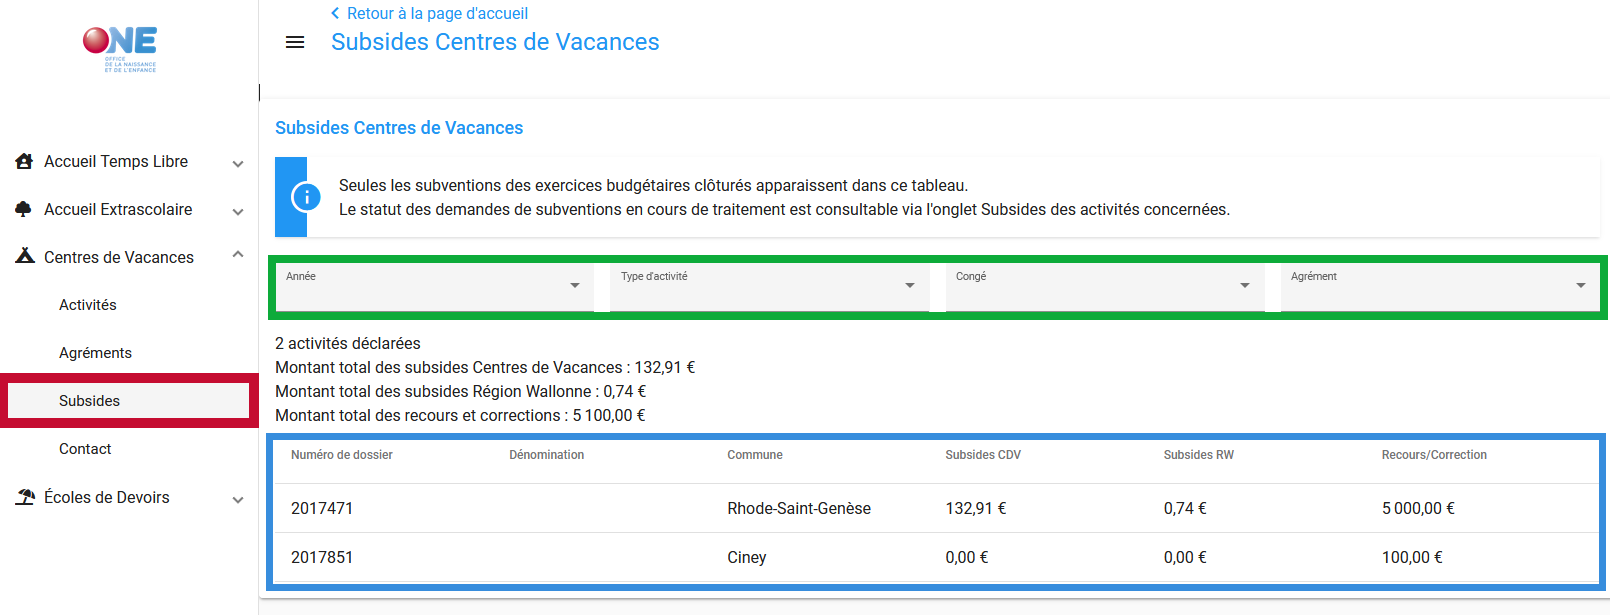
\includegraphics[width=14cm]{Images/cdv/cdv-ds-montants.png}
    \caption{Entrée subsides: vous avez la possibilité d'appliquer les filtres suivants: l'année de subvention, le type d'activité, le congé concerné (\textit{autrement dit, la période de vacances}) et/ou de sélectionner un agrément en particulier. }
    \label{fig:cdv_entrée_subsides}
\end{figure}


En cliquant sur la ligne d'un dossier en particulier, vous accéderez à l'onglet \ovalbox{subsides} de l'activité. Trois sous-onglets sont disponibles: 

\begin{itemize}
    \item \ovalbox{statut}: où vous pourrez prendre connaissance de la décision (octroi, octroi partiel ou refus), des lacunes et du commentaire de la décision; 
    \item \ovalbox{calcul}: pour avoir un détail du calcul du subside;
    \item \ovalbox{recours/correction}: en cas de contestation de la première décision, vous pourrez prendre connaissance de la décision concernant votre recours. Les éventuelles rectifications du montant du subside (en cas d'erreur par exemple) seront également disponibles.
\end{itemize}

\begin{figure}[h]
    \centering
    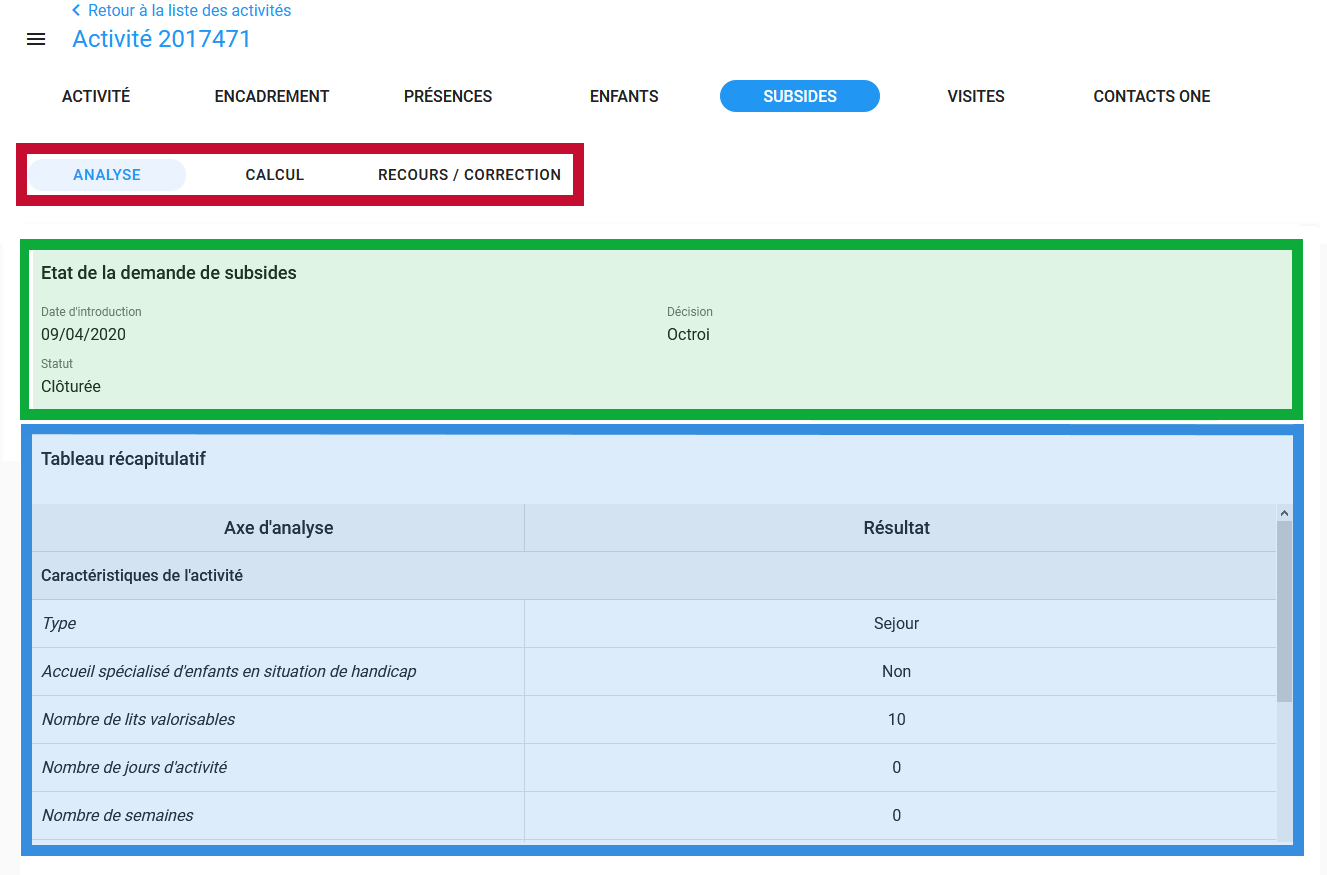
\includegraphics[width=16cm]{Images/cdv/cdv-ds-details.png}
    \caption{Onglet subsides: le détail du calcul de votre subvention est disponible dans le sous-onglet calcul.}
    \label{fig:cdv_onglet_subsides}
\end{figure}